\documentclass[12pt]{article}

\usepackage{times}
\usepackage{textcomp}
\usepackage{listings}
\usepackage{fullpage}
\usepackage{color}
\usepackage{hyperref} 
\usepackage{pst-tree} 
\usepackage{verbatim} 
\usepackage{graphicx}
\usepackage{amsmath,amsfonts,amssymb,amsthm}
\graphicspath{ {./}}


\def\part#1{\item[\bf #1)]}
\renewcommand{\thesubsection}{Question \arabic{subsection}}

\author{Clement Tsang}

\begin{document}

\begin{center}
    \Large\textbf{CS 241, Lecture 12 - Top-Down Parsing (cont.), LL(1), First and Follow}
\end{center}

\section{Warm Up Problem}
Consider the following grammar:
\begin{align*}
    S' \rightarrow \dashv S \vdash \qquad &(0)\\
    S \rightarrow bSd \qquad &(1)\\
    S \rightarrow pSq \qquad &(2)\\
    S \rightarrow C \qquad &(3)\\
    C \rightarrow rC \qquad &(4)\\
    C \rightarrow \epsilon \qquad &(5)
\end{align*}
Recall our definition of First($\beta$) is for \emph{non-terminals}, so in advance, we would not have $C$ in our First of $S$!  For Nullable, First, and Follow:\\\quad\\
\begin{tabular}{c||c|c|c}
    & Nullable & First & Follow \\
    \hline
    $S'$ & False & $\{\vdash\}$ & \{\} \\
    $S$ & True $(S \rightarrow C \rightarrow \epsilon)$ & $\{b, p, r\}$ & $\{\dashv, d, q\}$\\
    $C$ & True (rule 5) & $\{r\}$ & $\{\dashv, d, q\}$\\
\end{tabular}\\

\noindent For our predict table, recall that Predict($A, a$) = $\{A \rightarrow \beta: a \in First(\beta)\} \cup \{A \rightarrow \beta : \beta$ is nullable and $a \in Follow(A)\}$.  Thus:\\
\quad\\
\begin{tabular}{c||ccccccc}
    & $\vdash$ & $b$ & $d$ & $p$ & $q$ & $r$ & $\dashv$\\
    \hline
    $S'$ & \{0\}\\
    $S$ & & \{1\} & \{3\} & \{2\} & \{3\} & \{3\} & \{3\}\\
    $C$ & & & \{5\} & & \{5\} & \{4\} & \{5\}\\
\end{tabular}\\

\noindent We also see that this grammar is LL(1), as every entry has one element.  We'll drop the braces if we know it's LL(1), as there is only one entry in every cell.

\section{Top-Down Parsing (cont.)}
\begin{itemize}
    \item We note that for Nullable:
        \begin{itemize}
            \item $Nullable(\beta) = false$ whenever $\beta$ contains a terminal symbol.
            \item Further, $Nullable(AB) = Nullable(A) \wedge Nullable(B)$.
            \item Therefore, we can say that we only need to compute $Nullable(A)$ for all $A \in N'$.
            \item An algorithm to finding if a non-terminal symbol is Nullable is iterate a few times.  First, iterate through and change values.  Then again.  Our third iteration will determine if the symbol is truely Nullable.
            \item Example from slides:\\
                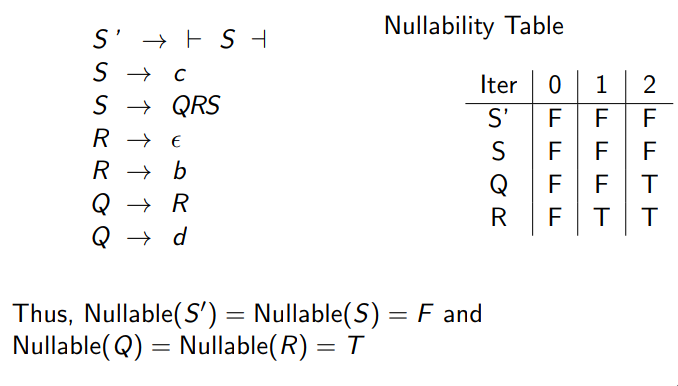
\includegraphics[scale=0.5]{nullable_alg.png}
        \end{itemize}
    \item We note that for First:
        \begin{itemize}
            \item The idea is to process $B_1B_2\dots B_k$ from a production rule until you encounter a terminal or non-nullable symbol, then go to the next rule.  Repeat until no changes.
            \item So first check $First(B_1)$, then if that is nullable, check $First(B_2)$, and then $First(B_3)$, and so on.  If, say, $B_1$ is nullable, then $First(B) = First(B_1) \cup First(B_2\dots B_k)$.
            \item We will state that $\epsilon \not\in First(A)$ for any $A \in N'$ as we state that $First(A) \subseteq \Sigma'$.
            \item Example from the slides:\\
                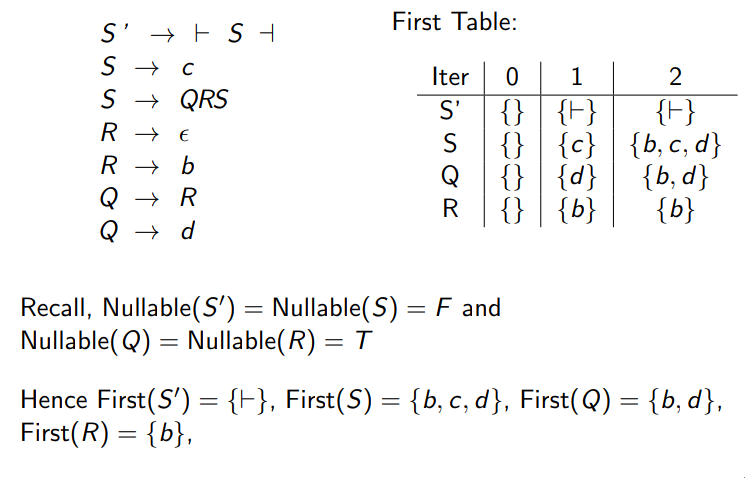
\includegraphics[scale=0.45]{first_alg.png}
        \end{itemize}
    \item For Follow:
        \begin{itemize}
            \item We will only look at the RHS of each rule.
            \item So, for example, if there was a rule $A \rightarrow B_1B_2$, then we use that to find $Follow(B_1)$.
            \item Another example is, say, $S \rightarrow QRS$.  Then we can find, from this rule, the Follow of $Q$ and $R$, where $Follow(Q) = First(R)$ or $First(S)$ if $R$ is nullable, and $Follow(R) = First(Q)$ or $First(Q)$ or $First(S)$, as $S \rightarrow QRS = QRQRS$.  
            \item Using that case, $Follow(B_1) = First(B_2) \cup Follow(A)$ if $B_2$ is nullable.
            \item Example:\\
                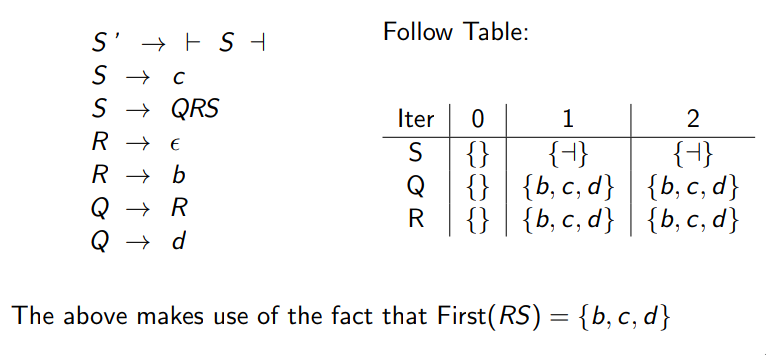
\includegraphics[scale=0.5]{follow_alg.png}
            \item In that example, we see that from rule (5), that $Follow(R) = Follow(Q) \cup Follow(R)$.  
        \end{itemize} 
\end{itemize}


\end{document}

